% Options for packages loaded elsewhere
\PassOptionsToPackage{unicode}{hyperref}
\PassOptionsToPackage{hyphens}{url}
%
\documentclass[
]{article}
\usepackage{lmodern}
\usepackage{amsmath}
\usepackage{ifxetex,ifluatex}
\ifnum 0\ifxetex 1\fi\ifluatex 1\fi=0 % if pdftex
  \usepackage[T1]{fontenc}
  \usepackage[utf8]{inputenc}
  \usepackage{textcomp} % provide euro and other symbols
  \usepackage{amssymb}
\else % if luatex or xetex
  \usepackage{unicode-math}
  \defaultfontfeatures{Scale=MatchLowercase}
  \defaultfontfeatures[\rmfamily]{Ligatures=TeX,Scale=1}
\fi
% Use upquote if available, for straight quotes in verbatim environments
\IfFileExists{upquote.sty}{\usepackage{upquote}}{}
\IfFileExists{microtype.sty}{% use microtype if available
  \usepackage[]{microtype}
  \UseMicrotypeSet[protrusion]{basicmath} % disable protrusion for tt fonts
}{}
\makeatletter
\@ifundefined{KOMAClassName}{% if non-KOMA class
  \IfFileExists{parskip.sty}{%
    \usepackage{parskip}
  }{% else
    \setlength{\parindent}{0pt}
    \setlength{\parskip}{6pt plus 2pt minus 1pt}}
}{% if KOMA class
  \KOMAoptions{parskip=half}}
\makeatother
\usepackage{xcolor}
\IfFileExists{xurl.sty}{\usepackage{xurl}}{} % add URL line breaks if available
\IfFileExists{bookmark.sty}{\usepackage{bookmark}}{\usepackage{hyperref}}
\hypersetup{
  pdftitle={Group\_07\_Analysis},
  pdfauthor={Group 7},
  hidelinks,
  pdfcreator={LaTeX via pandoc}}
\urlstyle{same} % disable monospaced font for URLs
\usepackage[margin=1in]{geometry}
\usepackage{graphicx}
\makeatletter
\def\maxwidth{\ifdim\Gin@nat@width>\linewidth\linewidth\else\Gin@nat@width\fi}
\def\maxheight{\ifdim\Gin@nat@height>\textheight\textheight\else\Gin@nat@height\fi}
\makeatother
% Scale images if necessary, so that they will not overflow the page
% margins by default, and it is still possible to overwrite the defaults
% using explicit options in \includegraphics[width, height, ...]{}
\setkeys{Gin}{width=\maxwidth,height=\maxheight,keepaspectratio}
% Set default figure placement to htbp
\makeatletter
\def\fps@figure{htbp}
\makeatother
\setlength{\emergencystretch}{3em} % prevent overfull lines
\providecommand{\tightlist}{%
  \setlength{\itemsep}{0pt}\setlength{\parskip}{0pt}}
\setcounter{secnumdepth}{5}
\usepackage{booktabs}
\usepackage{longtable}
\usepackage{array}
\usepackage{multirow}
\usepackage{wrapfig}
\usepackage{float}
\usepackage{colortbl}
\usepackage{pdflscape}
\usepackage{tabu}
\usepackage{threeparttable}
\usepackage{threeparttablex}
\usepackage[normalem]{ulem}
\usepackage{makecell}
\usepackage{xcolor}
\ifluatex
  \usepackage{selnolig}  % disable illegal ligatures
\fi

\title{Group\_07\_Analysis}
\author{Group 7}
\date{}

\begin{document}
\maketitle

\hypertarget{sec:Intro}{%
\section{Introduction}\label{sec:Intro}}

IMDb is a platform that provides information , ratings and reviews on
films, movies and many other streaming content. Our group was given a
dataset taken from this databese, which has records of 2387 films
released from \texttt{r\ min(film\$year)} to 2005 Each film has a unique
identification number (id) and some other measurments related to it.
Those are : \textbackslash begin \{itemize\}

\item

\$ Year\_i \$ : the year the film was released at cinemas

\item

\$ Length\_i \$ : duration of film in minutes

\item

\$ Budget\_i\$ : Budget for film production in\$ \$ 10\^{} 5 \$'s

\item

\$ Vote\_i \$ : Number of positive votes

\item

\$ Genre\_i \$ : Genre of film

\item

\$ Rating\_i \$ : IMDb rating from 1 to 10 \textbackslash end
\{itemiza\}

\hypertarget{sec:EDA}{%
\section{Exploratory Data Analysis}\label{sec:EDA}}

Taking a glance at the summaries of the variables shown in Table
\ref{tab:summary} we notice that length variable has many outliers , and
that is given by the big difference between its maximum value and its
third quartile value ,that is 399 minutes and 100 minutes respectively.
Budget also has a wide range of variability and an amount of outliers .
It is worth mentioning that votes have a large sandard deviation , 4370
to be exact and that might be because of an outlier that presents a huge
difference with the rest. Possibly a small number of films had
respectively huge number of votings compared to the rest of films.

\begin{table}[!h]

\caption{\label{tab:summary}\label{tab:summary}Summary statistics of variables in the data set.}
\centering
\fontsize{10}{12}\selectfont
\begin{tabular}[t]{lrrrrrrrr}
\toprule
Variable & Mean & SD & Min & Q1 & Median & Q3 & Max & IQR\\
\midrule
length & 81.414 & 37.675 & 1.0 & 72.0 & 90.0 & 100.0 & 399.0 & 10.0\\
budget & 11.948 & 2.968 & 2.1 & 10.0 & 12.0 & 13.9 & 23.7 & 1.9\\
votes & 658.969 & 4370.038 & 5.0 & 12.0 & 32.0 & 118.0 & 103854.0 & 86.0\\
rating & 5.414 & 2.069 & 0.7 & 3.7 & 4.7 & 7.8 & 9.2 & 3.1\\
\bottomrule
\end{tabular}
\end{table}

\begin{verbatim}
     rating     
 Min.   :0.700  
 1st Qu.:3.700  
 Median :4.700  
 Mean   :5.414  
 3rd Qu.:7.800  
 Max.   :9.200  
\end{verbatim}

\begin{figure}[H]

{\centering 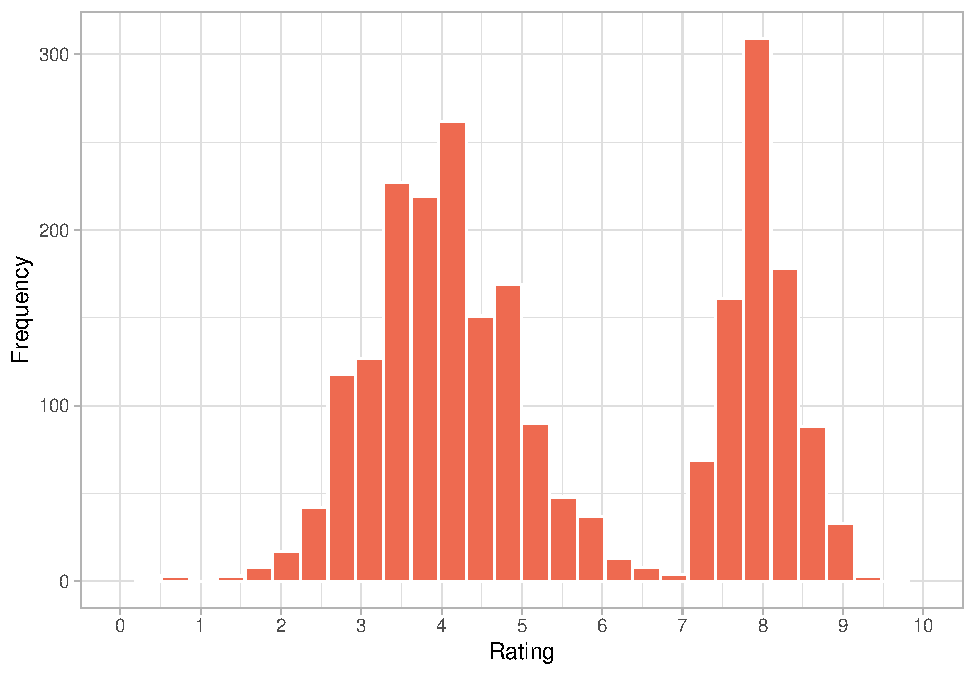
\includegraphics[width=0.68\linewidth]{Group_07_Analysis_files/figure-latex/ratings -1} 

}

\caption{\label{fig:ratings} Density Of Ratings}\label{fig:ratings }
\end{figure}

\begin{figure}[H]

{\centering 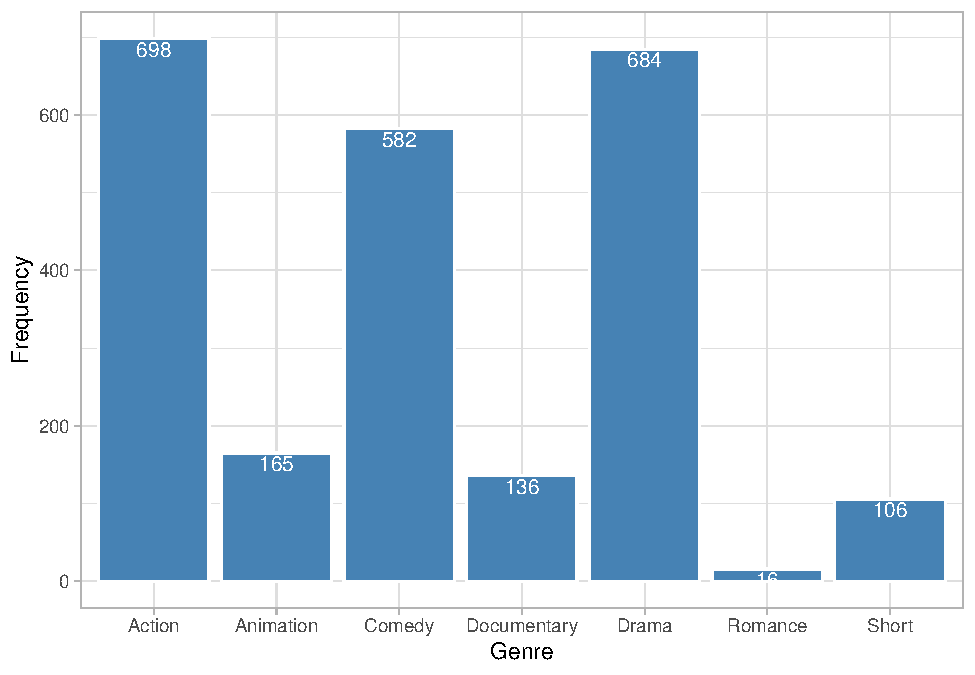
\includegraphics[width=0.68\linewidth]{Group_07_Analysis_files/figure-latex/genre -1} 

}

\caption{\label{fig:genre} Frequency of each genre.}\label{fig:genre }
\end{figure}

Given the barplot in Figure\ref{fig:genre} we notice that the majority
of films are within one of the 3 most dominant categories Action, Comedy
and Drama. On the opposite Animation Documentary and Short films have
relatively lower frequencies. Finaly Romance films are comparatively
very rare among our list of films ( only 16 films where Romantic among
all 2387)

\begin{table}[!h]

\caption{\label{tab:unnamed-chunk-1}\label{tab:summary}Summary statistics of variables in the data set.}
\centering
\fontsize{10}{12}\selectfont
\begin{tabular}[t]{llllllll}
\toprule
Rate & Action & Animation & Comedy & Documentary & Drama & Romance & Short\\
\midrule
<=7 & 37.4\% (578) & 3.3\%  (51) & 15.5\% (239) & 0.7\%  (11) & 42.0\% (650) & 1.0\% (16) & 0.1\%   (1)\\
>7 & 14.3\% (120) & 13.6\% (114) & 40.8\% (343) & 14.9\% (125) & 4.0\%  (34) & 0.0\%  (0) & 12.5\% (105)\\
\bottomrule
\end{tabular}
\end{table}

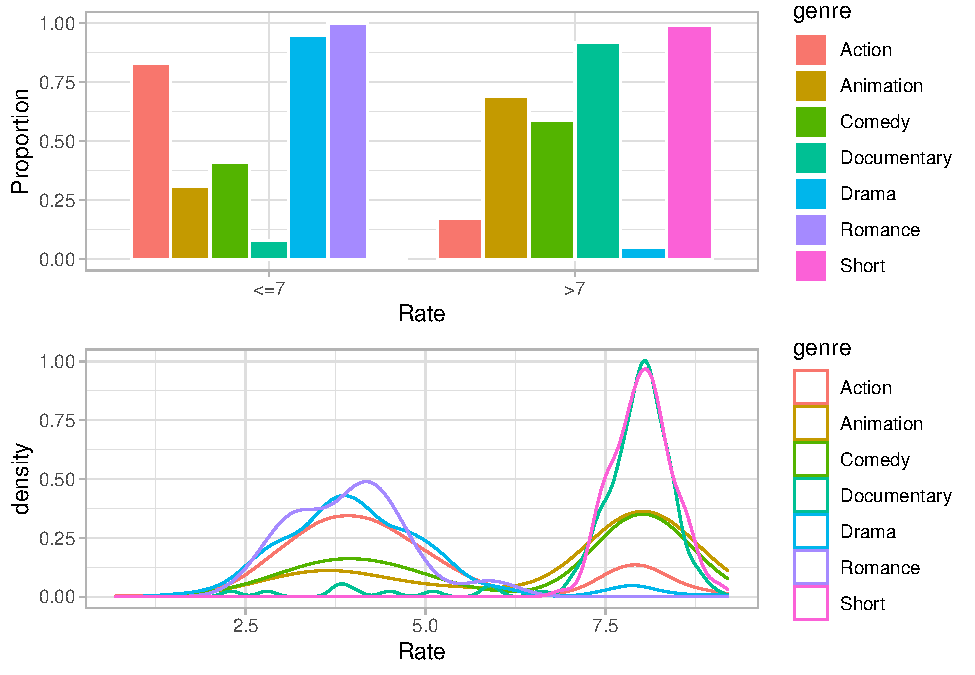
\includegraphics{Group_07_Analysis_files/figure-latex/unnamed-chunk-1-1.pdf}
\includegraphics{Group_07_Analysis_files/figure-latex/unnamed-chunk-1-2.pdf}

\begin{verbatim}
   Min. 1st Qu.  Median    Mean 3rd Qu.    Max. 
  2.700   3.300   4.050   3.950   4.275   5.900 
\end{verbatim}

From both the density graph and the barplot, we can see that
Short,Documentary,Comedy and Animation films are more likely to get
rates over 7.5 compared to rates given to Romance, Drama and Action
films,lower than 7 ( 5 to be exact ) In addition given the barchart we
notice that in our dataset all Romance films have ratings below 7. This
might indicate that Romance is not a strong explanation of rating.

\begin{figure}[H]

{\centering 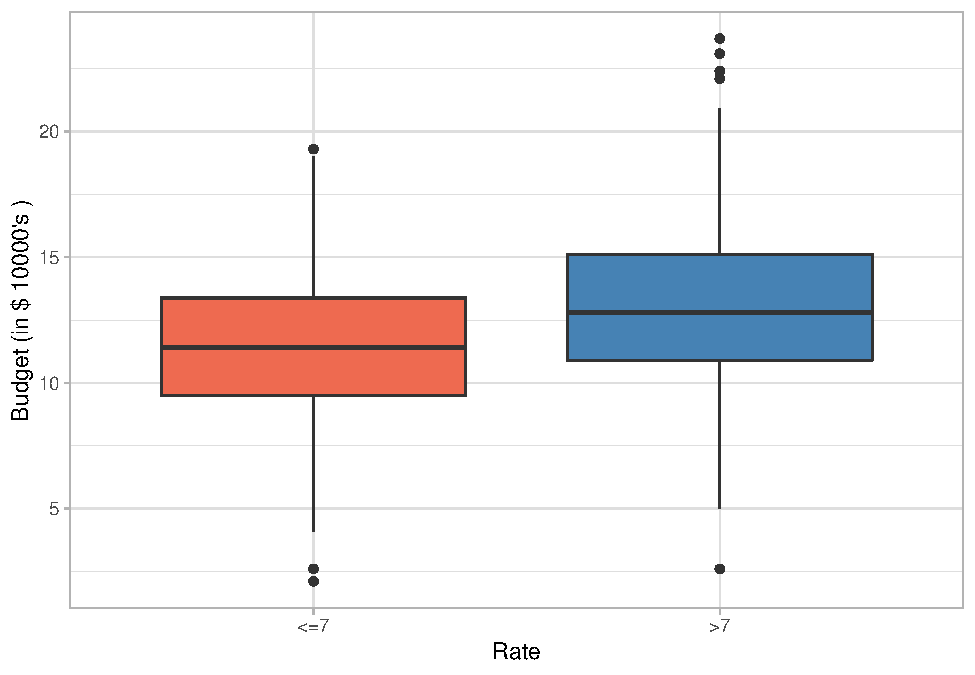
\includegraphics[width=0.68\linewidth]{Group_07_Analysis_files/figure-latex/budget-1} 

}

\caption{\label{fig:budget} Budget and Rate.}\label{fig:budget}
\end{figure}

\begin{verbatim}
   Min. 1st Qu.  Median    Mean 3rd Qu.    Max.    NA's 
   1.00   72.00   90.00   81.41  100.00  399.00      92 
\end{verbatim}

\begin{figure}[H]

{\centering \includegraphics[width=0.68\linewidth]{Group_07_Analysis_files/figure-latex/length -1} 

}

\caption{\label{fig:length} Rating based on length of the film.}\label{fig:length }
\end{figure}

Figure \ref{fig:length} shows that the length feature has many outliers.
That is explained by the large number of point graphed outsiede the
box.Those points represent films that have duration longer than 100
minutes which is our \(3^{rd}\) quartile. We have 455 outliers. Despite
the outliers we might assume that length has an effect on the rate since
for each group of rate the range of length is significantlly different.

\begin{figure}[H]

{\centering \includegraphics[width=0.68\linewidth]{Group_07_Analysis_files/figure-latex/year -1} 

}

\caption{\label{fig:year} Rating based on Year Of Release of the film}\label{fig:year -1}
\end{figure}
\begin{figure}[H]

{\centering \includegraphics[width=0.68\linewidth]{Group_07_Analysis_files/figure-latex/year -2} 

}

\caption{\label{fig:year} Rating based on Year Of Release of the film}\label{fig:year -2}
\end{figure}

Both plots suggest that the Year of release does not have a role in the
rating scale. First, Figure\ref{fig:year} graphs overlapping boxes which
indicates that there is no significant difference between the two groups
of rating scales based on the Year of release of the film. Also from the
second plot, the plot of rate over the years ,although it seems that
people tend to rate more films however the difference between giving a
rate over 7 and lower than 7 for different years of release did not
chamge dramatically. That also suggests that Year of release does not
explain the rating scale given to a film.

\begin{figure}[H]

{\centering \includegraphics[width=0.68\linewidth]{Group_07_Analysis_files/figure-latex/votes-1} 

}

\caption{\label{fig:votes} Rating based on Number of positive votes}\label{fig:votes-1}
\end{figure}
\begin{figure}[H]

{\centering \includegraphics[width=0.68\linewidth]{Group_07_Analysis_files/figure-latex/votes-2} 

}

\caption{\label{fig:votes} Rating based on Number of positive votes}\label{fig:votes-2}
\end{figure}

Taking into account the number of positive votes again does not help
identifying if a film is most probably getting a rate lower than 7 or
higher than 7 .

\includegraphics{Group_07_Analysis_files/figure-latex/corr-1.pdf}
\includegraphics{Group_07_Analysis_files/figure-latex/corr-2.pdf} We see
that in general films' duration are roughly in same range except
Animation and Short films. Both have comparatively smaller length . In
summary we do not observe any correlation between any of our continuous
explanatory variables as all have their pairwise correlation coefficient
lower than 0.4.

\hypertarget{sec:FDA}{%
\section{Formal Data Analysis}\label{sec:FDA}}

As we noticed from our exploratory analysis the genre Romance has no
significant explanation and thus we remove observations that are Romance
films. Also since we notices that length of the film might be a
significant property that can determine the rating scale we proceed and
remove observations that have missing values for length.

\begin{verbatim}
Call:
glm(formula = Rate ~ genre + length, family = binomial(link = "logit"), 
    data = No_Rom_films)

Deviance Residuals: 
    Min       1Q   Median       3Q      Max  
-2.9520  -0.5732  -0.2469   0.3724   4.1533  

Coefficients:
                  Estimate Std. Error z value Pr(>|z|)    
(Intercept)       1.832605   0.269055   6.811 9.67e-12 ***
genreAnimation   -0.257000   0.299480  -0.858 0.390809    
genreComedy       1.949419   0.143447  13.590  < 2e-16 ***
genreDocumentary  3.989061   0.373338  10.685  < 2e-16 ***
genreDrama       -1.576207   0.222284  -7.091 1.33e-12 ***
genreShort        3.499947   1.028800   3.402 0.000669 ***
length           -0.038875   0.002934 -13.250  < 2e-16 ***
---
Signif. codes:  0 '***' 0.001 '**' 0.01 '*' 0.05 '.' 0.1 ' ' 1

(Dispersion parameter for binomial family taken to be 1)

    Null deviance: 2969.3  on 2279  degrees of freedom
Residual deviance: 1669.8  on 2273  degrees of freedom
AIC: 1683.8

Number of Fisher Scoring iterations: 7
\end{verbatim}

\begin{verbatim}
Call:
glm(formula = Rate ~ year + genre + length + log(votes) + log(budget), 
    family = binomial(link = "logit"), data = No_Rom_films)

Deviance Residuals: 
    Min       1Q   Median       3Q      Max  
-3.6767  -0.4164  -0.1217   0.2800   4.4303  

Coefficients:
                   Estimate Std. Error z value Pr(>|z|)    
(Intercept)      -16.087566   6.158824  -2.612   0.0090 ** 
year               0.002248   0.003121   0.720   0.4714    
genreAnimation    -0.408295   0.347465  -1.175   0.2400    
genreComedy        2.587390   0.177937  14.541  < 2e-16 ***
genreDocumentary   4.800342   0.420246  11.423  < 2e-16 ***
genreDrama        -2.012599   0.255049  -7.891 3.00e-15 ***
genreShort         4.498479   1.084818   4.147 3.37e-05 ***
length            -0.054366   0.003847 -14.133  < 2e-16 ***
log(votes)         0.135498   0.041837   3.239   0.0012 ** 
log(budget)        5.618517   0.371527  15.123  < 2e-16 ***
---
Signif. codes:  0 '***' 0.001 '**' 0.01 '*' 0.05 '.' 0.1 ' ' 1

(Dispersion parameter for binomial family taken to be 1)

    Null deviance: 2969.3  on 2279  degrees of freedom
Residual deviance: 1307.1  on 2270  degrees of freedom
AIC: 1327.1

Number of Fisher Scoring iterations: 7
\end{verbatim}

\includegraphics{Group_07_Analysis_files/figure-latex/modelfull-1.pdf}
\includegraphics{Group_07_Analysis_files/figure-latex/modelfull-2.pdf}

\begin{table}
\centering
\begin{tabular}{l|r|r}
\hline
  & 2.5 \% & 97.5 \%\\
\hline
(Intercept) & -28.2312711 & -4.0712351\\
\hline
year & -0.0038589 & 0.0083841\\
\hline
genreAnimation & -1.0973435 & 0.2664512\\
\hline
genreComedy & 2.2445980 & 2.9425922\\
\hline
genreDocumentary & 4.0254977 & 5.6835086\\
\hline
genreDrama & -2.5314070 & -1.5290699\\
\hline
genreShort & 2.7694135 & 7.4476104\\
\hline
length & -0.0621528 & -0.0470581\\
\hline
log(votes) & 0.0536024 & 0.2177630\\
\hline
log(budget) & 4.9089531 & 6.3661856\\
\hline
\end{tabular}
\end{table}

\begin{verbatim}
     (Intercept)             year   genreAnimation      genreComedy 
    1.031000e-07     1.002250e+00     6.647825e-01     1.329503e+01 
genreDocumentary       genreDrama       genreShort           length 
    1.215519e+02     1.336409e-01     8.988034e+01     9.470857e-01 
      log(votes)      log(budget) 
    1.145107e+00     2.754806e+02 
\end{verbatim}

\begin{verbatim}
Call:
glm(formula = Rate ~ genre + length + votes + budget, family = binomial(link = "logit"), 
    data = No_Rom_films)

Deviance Residuals: 
    Min       1Q   Median       3Q      Max  
-3.7603  -0.4140  -0.1178   0.2720   4.1785  

Coefficients:
                   Estimate Std. Error z value Pr(>|z|)    
(Intercept)      -3.618e+00  4.428e-01  -8.170 3.09e-16 ***
genreAnimation   -1.974e-01  3.378e-01  -0.584   0.5590    
genreComedy       2.749e+00  1.835e-01  14.983  < 2e-16 ***
genreDocumentary  4.840e+00  4.098e-01  11.809  < 2e-16 ***
genreDrama       -2.040e+00  2.580e-01  -7.907 2.64e-15 ***
genreShort        4.209e+00  1.050e+00   4.009 6.11e-05 ***
length           -5.129e-02  3.566e-03 -14.382  < 2e-16 ***
votes             3.609e-05  1.672e-05   2.159   0.0309 *  
budget            4.962e-01  3.147e-02  15.770  < 2e-16 ***
---
Signif. codes:  0 '***' 0.001 '**' 0.01 '*' 0.05 '.' 0.1 ' ' 1

(Dispersion parameter for binomial family taken to be 1)

    Null deviance: 2969.3  on 2279  degrees of freedom
Residual deviance: 1290.1  on 2271  degrees of freedom
AIC: 1308.1

Number of Fisher Scoring iterations: 7
\end{verbatim}

\begin{verbatim}
Call:
glm(formula = Rate ~ genre + length + budget, family = binomial(link = "logit"), 
    data = film)

Deviance Residuals: 
    Min       1Q   Median       3Q      Max  
-3.7456  -0.4090  -0.1164   0.2675   4.1338  

Coefficients:
                   Estimate Std. Error z value Pr(>|z|)    
(Intercept)       -3.653590   0.441054  -8.284  < 2e-16 ***
genreAnimation    -0.151395   0.336400  -0.450    0.653    
genreComedy        2.748291   0.183255  14.997  < 2e-16 ***
genreDocumentary   4.804010   0.407660  11.784  < 2e-16 ***
genreDrama        -2.042906   0.256915  -7.952 1.84e-15 ***
genreRomance     -13.630907 314.185871  -0.043    0.965    
genreShort         4.237320   1.049719   4.037 5.42e-05 ***
length            -0.050386   0.003514 -14.340  < 2e-16 ***
budget             0.495057   0.031330  15.801  < 2e-16 ***
---
Signif. codes:  0 '***' 0.001 '**' 0.01 '*' 0.05 '.' 0.1 ' ' 1

(Dispersion parameter for binomial family taken to be 1)

    Null deviance: 2982.5  on 2294  degrees of freedom
Residual deviance: 1294.3  on 2286  degrees of freedom
  (92 observations deleted due to missingness)
AIC: 1312.3

Number of Fisher Scoring iterations: 14
\end{verbatim}

\hypertarget{sec:Conclude}{%
\section{Conclusion and further task}\label{sec:Conclude}}

\end{document}
